\documentclass[15pt,a5paper,reqno]{article}
\usepackage{hyperref}
\usepackage[warn]{mathtext}
\usepackage[utf8]{inputenc}
\usepackage[T2A]{fontenc}
\usepackage[russian]{babel}
\usepackage{amssymb, amsmath, multicol}
\usepackage{graphicx}
\usepackage[shortcuts,cyremdash]{extdash}
\usepackage{wrapfig}
\usepackage{gensymb}
\usepackage{floatflt}
\usepackage{lipsum}
\usepackage{verbatim}
\usepackage{concmath}
\usepackage{euler}
\usepackage{xcolor}
\usepackage{etoolbox}
\usepackage{fancyhdr}
\usepackage{subfiles}
\usepackage{enumitem}
\usepackage{amsthm}
\usepackage{indentfirst}
\usepackage{import}
\usepackage{multirow}

\DeclareMathOperator{\sign}{sign}

\RequirePackage[ left     = 1.5cm,
                 right    = 1.5cm,
                 top      = 2.0cm,
                 bottom   = 1.25cm,
                 includefoot,
                 footskip = 1.25cm ]{geometry}
                 
\setlength{\parskip}{ .5em plus .15em minus .08em }
\renewcommand {\baselinestretch}{ 1.07 }

\fancyhf{} % clear existing header/footer entries

\renewcommand{\footrulewidth}{ .0em }
\fancyfoot[C]{\texttt{\textemdash~\thepage~\textemdash}}

\makeatletter
\patchcmd\l@section{%
  \nobreak\hfil\nobreak
}{%
  \nobreak
  \leaders\hbox{%
    $\m@th \mkern \@dotsep mu\hbox{.}\mkern \@dotsep mu$%
  }%
  \hfill
  \nobreak
}{}{\errmessage{\noexpand\l@section could not be patched}}
\makeatother
\parindent = 1cm % отступ при красной строке⏎
\pagestyle{fancy}    
\renewcommand\qedsymbol{$\blacksquare$}

\newcommand{\when}[2]{
  \left. #1 \right|_{#2} \hspace
}
\renewcommand{\kappa}{\varkappa}
\RequirePackage{caption2}
\renewcommand\captionlabeldelim{}
\newcommand*{\hm}[1]{#1\nobreak\discretionary{}

\DeclareSymbolFont{T2Aletters}{T2A}{cmr}{m}{it}
{\hbox{$\mathsurround=0pt #1$}}{}}
% Цвета для гиперссылок
\definecolor{linkcolor}{HTML}{000000} % цвет ссылок
\definecolor{urlcolor}{HTML}{799B03} % цвет гиперссылок
 
\hypersetup{pdfstartview=FitH,  linkcolor=linkcolor,urlcolor=urlcolor, colorlinks=true}


\begin{document}

% НАЧАЛО ТИТУЛЬНОГО ЛИСТА
\begin{center}
  {\small ФЕДЕРАЛЬНОЕ ГОСУДАРСТВЕННОЕ АВТОНОМНОЕ ОБРАЗОВАТЕЛЬНОЕ\\ УЧРЕЖДЕНИЕ ВЫСШЕГО ОБРАЗОВАНИЯ\\ МОСКОВСКИЙ ФИЗИКО-ТЕХНИЧЕСКИЙ ИНСТИТУТ\\ (НАЦИОНАЛЬНЫЙ ИССЛЕДОВАТЕЛЬСКИЙ УНИВЕРСИТЕТ)\\ ФИЗТЕХ-ШКОЛА РАДИОТЕХНИКИ И КОМПЬЮТЕРНЫХ ТЕХНОЛОГИЙ}\\
  \hfill \break
  \hfill \break
  \hfill \break
  \Huge{Работа 3.2.5. \\ Вынужденные колебания в электрическом контуре}\\
\end{center}

\hfill \break
\hfill \break
\hfill \break
\hfill \break
\hfill \break
\hfill \break
\hfill \break
\hfill \break

\begin{flushright}
  \normalsize{Работу выполнил:}\\
  \normalsize{\textbf{Долгов Александр Алексеевич, группа Б01-106}}\\
\end{flushright}

\begin{center}
  \normalsize{\textbf{Долгопрудный, 2022}}
\end{center}

\thispagestyle{empty} % выключаем отображение номера для этой страницы

% КОНЕЦ ТИТУЛЬНОГО ЛИСТА

\newpage
\thispagestyle{plain}
\tableofcontents
\thispagestyle{plain}
\newpage

\section{Аннотация}

    В данной работе исследуются вынужденные колебания, возникающие в параллельном колебательном контуре под действием внешней гармонически меняющейся ЭДС.
	
\section{Теоретические сведения}

    Частота свободный гармонических колебаний в колебательном контуре:
    \begin{equation}\label{freq_0}
        \boxed{\nu_0 = \frac{1}{2\pi\sqrt{LC}}}
    \end{equation}

    \textbf{Добротность осциллятора} ($Q$) - отношение энергии, запасённой в осцилляторе к взятому со знаком минус изменению энергии системы при увеличении фазы на 1 радиан.
    \begin{equation}\label{Q_def}
        Q = \frac{E_0}{-\Delta E_1}
    \end{equation}

    Из уравнения затухающих колебаний можно получить следующую формулу, позволяющую вычислить добротность, зная параметры осциллятора:
    \begin{equation}\label{Q}
        Q = \frac{1}{1 - e^{-\frac{2\alpha}{\omega}}},
    \end{equation}
    где $\omega$ - частота колебаний осциллятора, $\alpha$ - коэффициент в уравнении затухающих колебаний ($\ddot x + 2\alpha\dot x + \omega_0^2 x = 0$), равный для колебательного контура $\frac{R}{2L}$. В случае $\alpha \ll \omega$ формула \eqref{Q} приводится к приближённому виду:
    \begin{equation}\label{Q_approx}
        \boxed{Q = \frac{\omega_0}{2\alpha} = \frac{1}{R}\sqrt{\frac{L}{C}}}
    \end{equation}
    Здесь применены разложение по формуле Тейлора до $o\left(\frac{2\alpha}{\omega}\right)$ и замена $\omega$ на $\omega_0$.

    \textbf{Ширина резонансной кривой} ($\Delta\omega$) - ширина области частот, в пределах которой энергия вынужденных колебаний уменьшается вдвое от значения энергии при резонансе.
    Воспользуемся формулой амплитуды установившихся вынужденных колебаний:
    \begin{equation}\label{voltage}
        U_m(\omega) = \frac{\mathcal{E}_0}{LC}\frac{1}{\sqrt{(\omega^2 - \omega_0^2)^2 + (2\alpha\omega)^2}}
    \end{equation}
    Из неё можно получить, что частота при резонансе равна:
    \begin{equation}\label{freq}
        \omega_{\text{р}} = \sqrt{\omega_0^2 - 2\alpha^2}
    \end{equation}
    Подставив \eqref{freq} в \eqref{voltage}, получим значение напряжения в резонансе:
    \begin{equation*}
        U_m(\omega_{\text{р}}) = \frac{\mathcal{E}_0}{RC}\frac{1}{\sqrt{\omega_0^2 - \alpha^2}}
    \end{equation*}
    Рассмотрим такие частоты $\omega_1$ и $\omega_2$ $(\omega_1 < \omega_2)$, что
    \[W(\omega_1) = W(\omega_2) = \frac{1}{2}W(\omega_{\text{р}}),\]
    тогда
    \[U_m(\omega_1) = U_m(\omega_2) = \frac{1}{\sqrt{2}} U_m(\omega_{\text{р}})\]
    Найдём эти частоты:
    \[\frac{\mathcal{E}_0}{LC}\frac{1}{\sqrt{(\omega_{1,2}^2 - \omega_0^2)^2 + (2\alpha\omega_{1,2})^2}} = \frac{1}{\sqrt{2}}\frac{\mathcal{E}_0}{RC}\frac{1}{\sqrt{\omega_0^2 - \alpha^2}}\]
    \[(\omega_{1,2} - \omega_0)^2(\omega_{1,2} + \omega_0)^2 + (2\alpha\omega_{1,2})^2 = 8\alpha^2(\omega_0^2 - \alpha^2)\]
    Далее предполагаем, что $\alpha \ll \omega_0$, тогда 1) $\omega_{1, 2} \approx \omega_0$, 2) $\omega_0^2 - \alpha^2 \approx \omega_0^2$. С учётом этих приближений имеем:
    \[(\omega_{1,2} - \omega_0)^2(2\omega_0)^2 + (2\alpha\omega_0)^2 = 8\alpha^2\omega_0^2\]
    \[(\omega_{1,2} - \omega_0)^2 = \alpha^2\]
    \[\omega_1 = \omega_0 - \alpha,\\\ \omega_2 = \omega_0 + \alpha\]
    Окончательно получаем:
    \begin{equation}\label{width}
        \Delta\omega = 2\alpha  
    \end{equation}
    Подставив \eqref{width} в \eqref{Q_approx}, получим:
    \begin{equation}\label{Q_width}
        \boxed{Q = \frac{\omega_0}{\Delta\omega} = \frac{\nu_0}{\Delta\nu}} 
    \end{equation}

    \textbf{Логарифмический декремент затухания} ($d$) - безразмерная величина, равная натуральному логарифму отношения двух последовательных амплитуд колеблющейся величины.
    \begin{equation*}
        d = \ln{\frac{A(t)}{A(t + T)}}
    \end{equation*}
    Для произвольных затухающих колебаний :
    \[d = \ln{\frac{A_0e^{-\alpha t}}{A_0e^{-\alpha(t + T)}}} = \ln{\frac{1}{e^{-\alpha T}}} = \alpha T\]
    \begin{equation}\label{decrement}
        \boxed{d = \alpha T}
    \end{equation}
    Выразив $\alpha$ из \eqref{decrement} и подставив её в \eqref{Q_approx}, получим связь между логарифмическим декрементом и добротностью:
    \begin{equation*}
        \boxed{Q = \frac{\pi}{d}}
    \end{equation*}

    Введём вспомогательную величину $d_n = \ln{\frac{A(t)}{A(t + nT)}},\ n\in\mathbb{N}$. Очевидно, что $d_n = nd$. Поэтому добротность через величину $d_n$ выражается следующим образом:
    \begin{equation}\label{Q_decrement}
        \boxed{Q = \frac{\pi n}{d_n}}
    \end{equation}
    
\section{Экспериментальная установка}

    Схема установки приведена на Рисунке 1.
    
    \begin{center}
        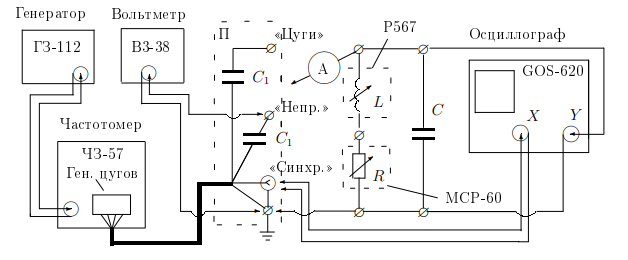
\includegraphics[width = \textwidth]{images/setup.png}
        \textbf{Рисунок 1. Схема экспериментальной установки}
    \end{center}

    Синусоидальный сигнал от звукового генератора проходит через частотометр, позволяющий измерять рабочую частоту. В корпус частотометра вмонтирован генератор цугов - электронное реле, разрезающее синусоиду на периодически повторяющиеся цуги - отрезки синусоиды, содержащие 32 или 40 периодов колебаний.

    Затем сигнал (цуги или непрерывный сигнал) поступает по коаксильному кабеля (по отдельным каналам) через одинаковые конденсаторы ёмкостью $C_1 \approx 600\text{ пкФ}$ на клеммы "цуги"\ или "непр."\ , вмонтированные на отдельной панели П. На ней также смонтированы клеммы "синхр."\ (синхронизация) и "$\perp$"\ (земля). При подключении контура к клеммам "непр." и "$\perp$"\ на контур подаётся непрерывный сигнал; если контур подключён к клеммам "цуги" и "$\perp$"\ - на контур подаются отрезки синусоиды.

    Для визуального наблюдения за процессом колебаний напряжение с конденсатора подаётся на вход электронного осциллографа (ЭО). Для устойчивости картины на экране ЭО его частота развёртки принудительно синхронизуется с частотой повторения цугов.
    
\section{Приборы и инструментальные погрешности}

    \noindent\textbf{Магазин сопротивлений:}\\
        Абсолютная погрешность: $\sigma_R = 0.005\text{ Ом}$

    \noindent\textbf{Амперметр:}\\
        Абсолютная погрешность: $\sigma_I = 0.05\text{ А}$

    \noindent\textbf{Вольтметр:}\\
        Абсолютная погрешность: $\sigma_U = 2\text{ мВ}$

    \noindent\textbf{Частотометр:}\\
        Абсолютная погрешность: $\sigma_{\nu} = 0,5\text{ Гц}$

    \noindent\textbf{Ёмкость конденсатора:} $C = (0.100 \pm 0.003)\text{ мкФ}$

    \noindent\textbf{Индуктивность катушки:} $L = (100.0 \pm 0.2)\text{ мГн}$

\section{Измерения и обработка их результатов}

    \subsection{Исследование резонансных кривых}

        Перед проведением измерений было получено теоретически предсказываемое значение собственной частоты колебаний в контуре. Оно находилось по формуле \eqref{freq_0}:
        \[\boxed{\nu_{0}^{(th)} = (1592\pm24)\text{ Гц}}\]

        Было проведено 2 серии по 7 измерений действующих значений напряжения и силы тока в контуре при различных частотах входного напряжения. В первой серии активное сопротивление, выставленное на магазине сопротивлений, равнялось $0,01\text{ Ом}$; во второй - $100\text{ Ом}$. Результаты измерений представлены в \hyperlink{table_1}{Таблице 1}. По этим данным также построены \hyperlink{graph_1}{График 1} (в относительных единицах по осям) и \hyperlink{graph_2}{График 2} (в абсолютных единицах по осям). Договоримся, что все величины, связанные с резонансной кривой, на которой $R = 0,01\text{ Ом}$, будем указывать с индексом 1; для второй кривой - с индексом 2.
        
        \noindentИз \hyperlink{graph_2}{Графика 2} можно получить ширину резонансных кривых:
        \[\boxed{\Delta\nu_1 = 60,4\text{ Гц}}\\\ \boxed{\Delta\nu_2 = 223,1\text{ Гц}}\]
        и собственную частоту колебаний:
        \[\boxed{\nu_0 = (1551,0 \pm 0,5)\text{ Гц}}\]
        Добротность колебательного контура найдём по формуле \eqref{Q_width}:
        \[\boxed{Q_1 = 25,6788}\\\ \boxed{Q_2 = 6,952}\]

        Теоретическое значение добротности может быть найдено по формуле \eqref{Q_approx}, а погрешность по формуле:
        \[\sigma_Q = Q\sqrt{\left(\frac{\sigma_R}{R}\right)^2 + \left(\frac{\sigma_L}{2L}\right)^2 + \left(\frac{\sigma_C}{2C}\right)^2}\]
        Итак, теоретически добротность данного контура равна:
        \[\boxed{Q_1^{(th)} = (1 \pm 0,5)\cdot 10^5}\\\ \boxed{Q_2^{(th)} = 10,0 \pm 0,2}\]

    \subsection{Процессы установления и затухания колебаний}

        Для каждого из сопротивлений $R = 0,01\text{ Ом}$ и $R = 100\text{ Ом}$ было проведено 2 серии по 5 измерений. Каждое измерение первой серии заключалось в нахождении 2 амплитуд напряжения, разделённых некоторым числом периодов, при установлении вынужденных колебаний. Вторая серия предполагала измерение тех же величин, но уже для затухающих колебаний. Результаты приведены в \hyperlink{table_2}{Таблице 2}. По этим данным можно рассчитать добротность колебательного контура, используя формулу \eqref{Q_decrement}. Значения добротности также представлены в \hyperlink{table_2}{Таблице 2}.
        
        \noindentСредние значения добротности для случа затухания:
        \[\boxed{\overline{Q_1} = 29,2}\\\ \boxed{\overline{Q_2} = 8.1}\]
        Погрешность величину $d_n$ находится по формуле:
        \[\sigma_{d_n} = \sigma_U\sqrt{\frac{1}{U_k^2} + \frac{1}{U_{k+n}^2}}\]
        Погрешность добротности находится по формуле:
        \[\sigma_Q = \frac{\pi n}{d_n^2}\sigma_{d_n} = Q\sqrt{\frac{1}{U_k^2} + \frac{1}{U_{k+n}^2}}\frac{\sigma_U}{d_n}\]
    
\section{Вывод}

        
    
\newpage
\section{Приложения}

    \subsection{Таблицы}

    \noindent\hypertarget{table_1}{\textbf{Таблица 1. Исследование резонансных кривых}}
    \begin{center}
        \begin{tabular}{|c|c|c|c|c|c|c|c|}
            \hline
            \multicolumn{3}{|c|}{\textbf{R = 0,01 \text{Ом}}} & \multicolumn{3}{|c|}{\textbf{R = 100 \text{Ом}}} \\ \hline\hline
            $\nu$, Гц & I, А  & U, мВ  & $\nu$, Гц & I, А  & U, мВ \\ \hline\hline
                 1556 & 22,23 & 175    &      1551 & 21.40 & 54    \\ \hline
                 1566 & 19,48 & 160    &      1608 & 21.11 & 50    \\ \hline
                 1573 & 18,36 & 150    &      1652 & 21.41 & 42    \\ \hline
                 1580 & 17,72 & 130    &      1695 & 22.00 & 36    \\ \hline
                 1590 & 17,66 & 110    &      1752 & 22.92 & 30    \\ \hline
                 1606 & 18,23 &  90    &      1808 & 23.81 & 26    \\ \hline
                 1627 & 19,17 &  70    &      1888 & 25.07 & 22    \\ \hline
                 1551 & 23.47 & 175    &      1558 & 21.30 & 54    \\ \hline
                 1536 & 25.91 & 155    &      1503 & 21.60 & 48    \\ \hline
                 1528 & 26.08 & 135    &      1490 & 21.55 & 44    \\ \hline
                 1521 & 25.87 & 120    &      1466 & 21.34 & 40    \\ \hline
                 1518 & 25.26 &  95    &      1434 & 20.92 & 34    \\ \hline
                 1494 & 24.37 &  75    &      1408 & 20.52 & 30    \\ \hline
                 1487 & 23.94 &  70    &      1380 & 20.06 & 26    \\ \hline
        \end{tabular}
    \end{center}

    \newpage
    \noindent\hypertarget{table_2}{\textbf{Таблица 2. Установление и затухание колебаний}}
    \begin{center}
        \begin{tabular}{|c|c|c|c|c|c|c|c|c|c|}
            \hline
            \multicolumn{5}{|c|}{\textbf{R = 0,01 \text{Ом}}} & \multicolumn{5}{|c|}{\textbf{R = 100 \text{Ом}}} \\ \hline\hline
            $U_k, \text{мВ}$ & $U_{k + n}, \text{мВ}$ & n & $d_n$ & Q & $U_k, \text{мВ}$ & $U_{k + n}, \text{мВ}$ & n & $d_n$ & Q\\ \hline\hline
            \multicolumn{10}{|c|}{\text{Установление колебаний}}            \\ \hline
               200 & 400 & 8 & -0.7  & 36  &      40 & 100 & 2 & -0.9  & 7  \\ \hline
               100 & 120 & 1 & -0.18 & 17  &      40 & 130 & 5 & -1.2  & 13 \\ \hline
               280 & 400 & 6 & -0.36 & 52  &     100 & 140 & 6 & -0.34 & 55 \\ \hline
               440 & 480 & 5 & -0.09 & 170 &      70 & 120 & 3 & -0.54 & 17 \\ \hline
               300 & 420 & 7 & -0.34 & 65  &     110 & 130 & 2 & -0,17 & 37 \\ \hline
            \multicolumn{10}{|c|}{\text{Установившееся напряжение}}  \\ \hline
            \multicolumn{5}{|c|}{500 \text{ мВ}} & \multicolumn{5}{|c|}{140 \text{ мВ}} \\ \hline
            \multicolumn{10}{|c|}{\text{Затухание колебаний}}       \\ \hline
               420 & 380 & 1 & 0.10 & 30   &     110 & 70 & 1 & 0.45 & 7\\ \hline
               340 & 220 & 4 & 0.44 & 29   &      50 & 20 & 2 & 0.9  & 7\\ \hline
               300 & 200 & 4 & 0.41 & 31   &      70 & 20 & 3 & 1.3  & 7.3\\ \hline
               380 & 160 & 8 & 0.86 & 29   &      50 & 10 & 5 & 1.6  & 10\\ \hline
               200 & 100 & 6 & 0.7  & 27   &      10 & 10 & 7 & 2.4  & 9.2\\ \hline
        \end{tabular}
    \end{center}

    \subsection{Графики}

    \noindent\hypertarget{graph_1}{\textbf{График 1. Резонансный кривые (относительные величины)}}
    \begin{center}
        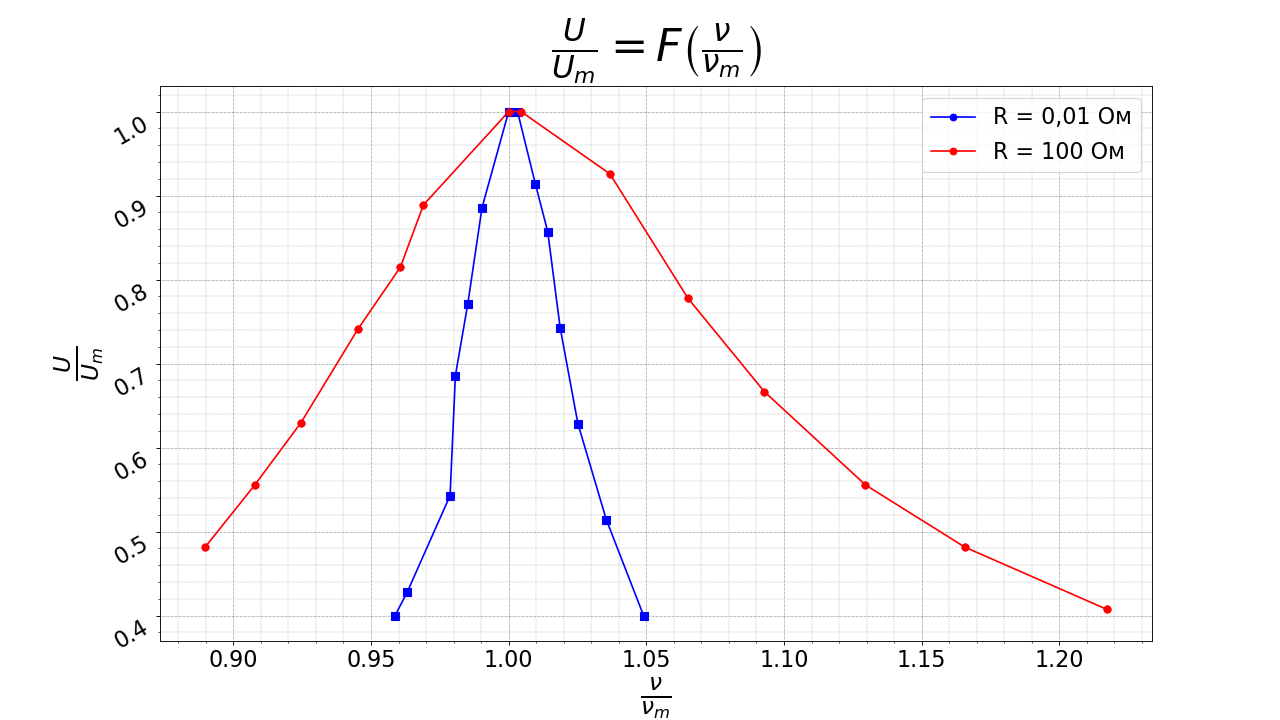
\includegraphics[width = \textwidth]{images/graph_1.png}
    \end{center}
    \noindent\hypertarget{graph_2}{\textbf{График 2. Резонансный кривые (абсолютные величины)}}
    \begin{center}
        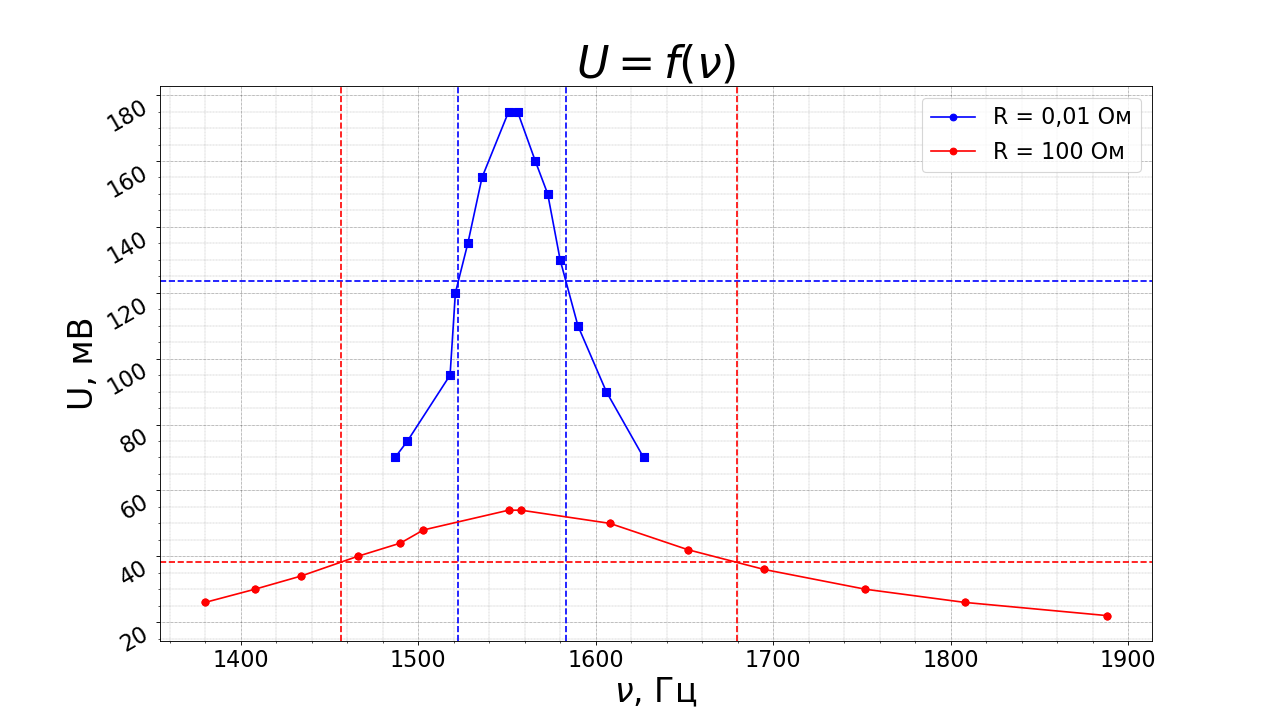
\includegraphics[width = \textwidth]{images/graph_2.png}
    \end{center}


\end{document}